\documentclass{article}
\usepackage[utf8]{inputenc}
\usepackage[czech]{babel}
\usepackage{graphicx}
\clubpenalty=1000
\widowpenalty=1000
\hyphenpenalty=500
\tolerance=3000

\title{Raketka - programátorská dokumentace}
\author{Kateřina Nevolová \\ \texttt{katka.nevolova@gmail.com} \\ I-Y-40, 73502469}

\begin{document}
\maketitle

Raketka je jednoduchá hra pro linux napsaná v jazyce C za pomocí knihoven GLUT
a OpenGL pro grafiku. Program se sestává z několika modulů, z nichž se většina stará o nějaký konkretní subsystém. Veškeré napojení na GLUT a hlavní cyklus programu je popsán v modulu main, který se dále odkazuje na game obstarávající herní
logiku. Většina modulů pak sdílí společný formát:

\begin{itemize}
\item inicializační a deinicializační funkci
\item funkci pro posun herního stavu o nějaký časový úsek
\item případně funkci pro vykreslení pomocí OpenGL
\item lokální data uložená v globální proměnné, často spojovém seznamu
\end{itemize}

\section{Soupis modulů}

\subsection{main.c}
Obsahuje funkci main s GLUTovými funkcemi pro vytvoření a obsluhování
OpenGL okna apod., sbírá a pamatuje si klávesnicový vstup. Snímá
přesný čas hry a předává ho dál herní logice do modulu game.
Periodicky vyvolává překreslení scény.

\subsection{game.c}
Inicializuje všechny součásti hry. Pamatuje si level hry a power
level hráče, funkcí \texttt{handle\_levels} komunikuje s modulem enemy (funkce
\texttt{out\_of\_enemies}), popřípadě dá vědět modulu enemywave
(\texttt{generate\_enemy\_wave}) pro nagenerování nové vlny nepřátel. Funkce
\texttt{draw\_game} kreslí celou hru, a v případě hráčovy smrti i koncový
screen hry. Dále komunikuje s modulem text funkcemi \texttt{draw\_string} a
\texttt{draw\_int} pro výpis statistik hry. Funkce \texttt{update\_game} posune
všechny herní součásti o specifický časový interval a zpracovává
klávesnicový vstup z modulu main (funkce \texttt{k\_left}, \texttt{k\_right}, \texttt{k\_up},
\texttt{k\_down} a \texttt{k\_fire}). V případě hráčovy smrti dává možnost spustit hru
znovu. Pomocí funkcí \texttt{player\_injury} a \texttt{player\_exposion} se stará
o particlové efekty (funkce \texttt{add\_particle} z modulu particles) při
kontaktu střely s raketkou. Funkce \texttt{try\_to\_damage\_player} poskytuje
informaci o stavu hráče modulu bullets, popřípadě volá funkce
\texttt{player\_injury} a \texttt{player\_explosion}. Funkce \texttt{player\_bonuses} předává
informace o lapení bonusu modulu bonus. A konečně funkce \texttt{add\_score}
přidává skóre.

\subsection{enemy.c}
Spojový seznam \texttt{struct e} uchovává pozici, rychlost, životy a další
parametry nepřátel. Jednoduchá nepřátelská inteligence je ve funkci
\texttt{enemy\_ai}, např. přidávání střel do modulu bullets. Kolize se
střelami jsou ošetřovány funkcí \texttt{try\_to\_damage\_enemy}, která případně
smaže nepřítele, udělá výbuch (\texttt{make\_exposion}) z particlů, přidá
skóre (\texttt{add\_score} z modulu game) a případně nechá vypadnout bonus
(\texttt{add\_bonus} z modulu bonus). Funkci \texttt{out\_of\_enemies} používá modul
game, aby zjistil jestli je potřeba přidat další nepřátele.

\subsection{enemywave.c}
Obsahuje jednoduchou funkci \texttt{generate\_enemy\_wave} volanou z modulu
game na začátku každého levelu na vytvoření skupinky nepřátel. Toto je
hlavní místo, kde by bylo dobré hru ještě vylepšit, speciálně by bylo
potřeba udělat levely zajímavější (navzájem odlišnější).

\subsection{bullets.c}
Spojový seznam \texttt{struct b} se střelami různých typů, původu (přátelské,
nepřátelské), pozicí, rychlostí a způsobovaným poškozením. Pomocí
funkcí \texttt{try\_to\_damage\_enemy} z modulu enemy a \texttt{try\_to\_damage\_player} z modulu game zjišťuje kolizi s obětí.

\subsection{bonus.c}
Spojový seznam \texttt{struct b} s padajícími power-upy několika barev.
Pomocí funkce \texttt{player\_bonuses} z modulu game zjišťuje jestli hráč
bonus zrovna nesebral.

\subsection{particles.c}
Modul pro kreslení částicového systému (explozí apod.). Všechny
částice jsou uložené ve spojovém seznamu typu \texttt{struct s}, každá má
svoji pozici, rychlost (směr), barvu, trvanlivost a jeden ze tří
předem určených tvarů.

\subsection{background.c}
Kreslí ubíhající vesmír na pozadí složený z hvězd různé vzdálenosti.

\subsection{text.c}
Jednoduchý nástroj pro kreslení textu, font je ručně poskládaný z
vektorů.

\section{Kompilace a spuštění hry}

Ke kompilaci jsou potřeba knihovny GLUT a OpenGL. Program se sestaví pomocí
Makefile příkazem \texttt{make}. Skompilovaný program je poté připraven ke
spuštění příkazem \texttt{./raketka}.

\section{Screenshot s popisem}
\begin{center}
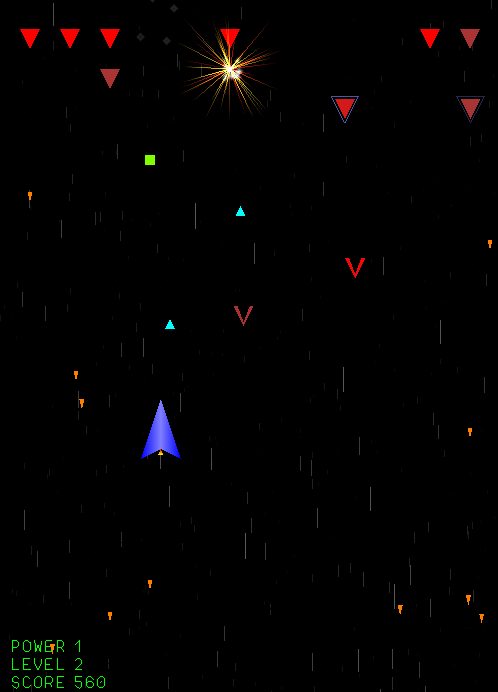
\includegraphics[width=7cm]{basic_hit.png}
\end{center}

Hráče (modrou raketku) ovládáme šipkami a vykresluje ho modul game, který také pomocí fontů z modulu text kreslí informace o hře (power level (životy/síla hráče), herní level a skóre) vlevo dole. Oranžové a modré střely vykresluje model bullets. Zelená krychlička je bonus (konkrétně dočasný upgrade útoku). Pohyblivé pozadí z bílých čar vykresluje modul background. Nahoře uprostřed můžeme sledovat exlpozi z particlů. Nepřátelé jsou červené trojúhelníky, přičemž modře obtažení mají vylepšený štít (více hp) a ti ve tvaru červeného V rychleji létají a střílí.

\end{document}
